\documentclass{beamer}
\usepackage{ctex} %注意这个宏包
\usepackage{color}
\usepackage{graphics,graphicx}
%\usetheme{Boadilla}
\usetheme{Hannover}
\usepackage{graphics,graphicx}
\usepackage{pstricks,pst-node,pst-tree}
\usecolortheme{crane}
\CTEXoptions[today=old]
\setCJKmainfont[BoldFont={SimHei},ItalicFont={KaiTi}] {WenQuanYi Micro Hei Mono}
\title{Introduction to Hidden Markov Model\\ 隐式马尔可夫模型}
\author{严春伟}
\institute[PKUSZ]{
    互联网研发中心\\
}
\date{\today}

\begin{document}
% ------------- title page ----------------------------
%--- the titlepage frame -------------------------%
\begin{frame}
  \titlepage
\end{frame}

\begin{frame}
\frametitle{Outline}
\tableofcontents
\end{frame}

\section{Introduction}
\begin{frame}{Introduction}
\begin{center}
$
\psmatrix[colsep=1cm,rowsep=1cm,mnode=circle]
q_1 & q_2 & q_3 & \cdots & q_T\\
s_1 & s_2 & s_3 & \cdots & s_T
% q -> s
\ncline{->}{1,1}{2,1}
\ncline{->}{1,2}{2,2}
\ncline{->}{1,3}{2,3}
\ncline{->}{1,5}{2,5}
% q -> q
\ncline{->}{1,1}{1,2}
\ncline{->}{1,2}{1,3}
\ncline{->}{1,3}{1,4}
\ncline{->}{1,4}{1,5}
\endpsmatrix
$
\end{center}

\begin{itemize}
\item a Markov process with unobserved (hidden) states
\item state is not directly visible
\item output, depend on the states, is visible
\end{itemize}
\end{frame}

\begin{frame}{HMM Uses}
\begin{itemize}
\item Speech recognition
    \begin{itemize}
    \item Recognizing spoken words and phrases
    \end{itemize}
\item Text processing
    \begin{itemize}
    \item Parsing raw records into structured records
    \end{itemize}
\item Bioinformatics
    \begin{itemize}
    \item Protein sequence prediction
    \end{itemize}
\item Financial
    \begin{itemize}
    \item Stock market forecasts (price pattern prediction)
    \item Comparison shoing services
    \end{itemize}
\end{itemize}
\end{frame}

\section{HMM Overview}
\begin{frame}{HMM Overview}
\begin{itemize}
\item Machine learning method
\item Makes use of state machines
\item Based on probabilistic models
\item Useful in problems having sequential steps
\item Can only observe output from states, not the states themselves
\end{itemize}
\end{frame}


\begin{frame}{Sepcifaction of an HMM}
    \begin{block}{definition}
        Full HMM is thus specified as a triplet:\\
        $\lambda = (N,M,A,B,\pi)$
    \end{block}

    \begin{block}{States}
    N--number of states
    \begin{itemize}
    \item Q=$\{ q_1, q_2, \cdots, q_T \}$
    \end{itemize}
    \end{block}

    \begin{block}{Symbols}
    M -- number of symbols
    \begin{itemize}
    \item O=$\{ o_1, o_2, \cdots, o_T \}$
    \end{itemize}
    \end{block}
\end{frame}

\begin{frame}{Sepcifaction of an HMM}
    \begin{block}{Transition Probility}
        \begin{itemize}
        \item A - the state transition probability matrix
            \begin{itemize}
            \item $a_{ij} = P(q_{t+1} = j | q_{t}=i)$
            \end{itemize}
        \end{itemize}
    \end{block}

    \begin{block}{Observation Probability}
        \begin{itemize}
        \item B- observation probability distribution
            \begin{itemize}
            \item $b_j{(k)} = P(O_t=k|q_t=j)$
            \end{itemize}
        \end{itemize}
    \end{block}
    
    \begin{block}{Initial State Distribution}
        \begin{itemize}
        \item $\pi$ -- the initial state distribution
        \end{itemize}
    \end{block}
\end{frame}


\section{Three basic problems of HMMs}
\begin{frame}[t]{Three basic problems of HMMs}
    Given an HMM $\lambda$ and a sequence of observations $O=o_1,o_2,\cdots,o_T$
    \begin{block}{1.\quad The Evaluation Problem}
     what is the probability that the observations are generated by the model, $P(O|\lambda)$? 
    \end{block}

    \begin{block}{2.\quad The Decoding Problem}
    what is the most likely state sequence in the model that produced the observations?
    \end{block}

\end{frame}
    

\begin{frame}{Three basic problems of HMMs}
    \begin{block}{3.\quad The Study Problem}
     how should we adjust the model parameters $\{\lambda, A, B\}$ in order to maximize $P(O|\lambda)$
    \end{block}
\end{frame}

\section{A concrete example}
\begin{frame}{A concrete example}
    \begin{block}{Case Description}
        \begin{itemize}
        \item Alice and Bob, who live far apart from each other
        \item Bom is only interested in three activities: walk, shop,clean.
        \item Bom's choice is exclusively based on the weather.
        \item Alice tries to guess what the weather is like there.
        \end{itemize}
    \end{block}
\end{frame}

\begin{frame}{A concrete example}
    \begin{center}
    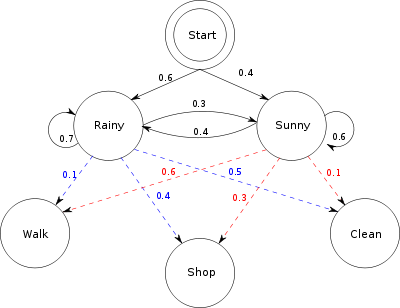
\includegraphics[height=150pt]{400px-HMMGraph.svg.png}
    \end{center}
\end{frame}

\begin{frame}{A concrete example}
    \begin{block}{Find the Most Likely Sequence of Hidden States}
    \begin{itemize}
    \item get Bom's activities : $\{ walk, walk, clean, run  \}$
    \item trying to guess the most likely weather sequence there
    \end{itemize}
    \end{block}

    \begin{block}{Soluction}
    \begin{enumerate}
    \item Forward Algorithm
    \item Back Algorithm
    \item Viterbi Algorithm
    \end{enumerate}
    \end{block}
    
\end{frame}

\section{References}
\begin{frame}{References}
\begin{thebibliography}{10}
\bibitem{HMM} [SR Eddy,Current opinion in structural biology, 1996]
    \newblock \emph{Hidden markov models}
\bibitem{HMM} [L Rabiner, B Juang - ASSP Magazine, IEEE, 1986]
    \newblock \emph{An introduction to hidden Markov models}
\bibitem{HMM} [李航,清华大学出版社]
    \newblock \emph{统计学习方法}
\end{thebibliography}
\end{frame}

\end{document}

